\newpage
\section{Input files and the databases}

\subsection{the .gpvdm simulation file format}
\label{sec:gpvdmfileformat}
This is a zip file, if you rename the file to .zip you will be able to open the file and in the file you will see a sim.json file.  You can view this file in any text editor but the file is quite complex and long so I recommend you use firefox to view it as it has a built in json viewer.  If you make a copy of this file outside the .gpvdm archive, gpvdm will ignore the sim.json file within the sim.gpvdm archive and revert to the plain text file stored in the simulation directory.  This feature can be useful for automation of simulations.

\subsection{Databases}
There are a series of databases used to define material parameters, shapes, emission spectra and solar spectra etc...  These are described within this section.  There are two copies of these databases, one copy in the install directory of gpvdm  C:$\backslash$Program Files$\backslash$gpvdm$\backslash$ and one in your home directory in a folder called gpvdm\_local.   When the model starts for the first time it copies the read only materials database from, to the gpvdm\_local folder in your home directory.  If you delete the copy of the materials database in the gpvdm\_local folder it will get copied back next time you start the model, this way you can always revert to the original databases if you damage the copy in gpvdm\_local.

The structure of the databases are simple, they are a series of directories with one directory dedicated to each material or spectra etc.. E.g. there will be one directory called Ag in the optical database which defines silver, and another directory in the spectra database called am1.5g which defines the solar spectrum.  Each of these database directories will from now on be referred to an object.  Within each object there is a data.json file which defines basic material properties and configuration information.  There will may be a couple of .bib files which contain reference information for the object in bibtex format and either .gmat files for n/k spectral data or .inp files for other types of data.  All these files are just human readable text files, so you can open them in your preferred text editor such as notepad.

\subsubsection{Materials database}
\label{sec:materialdatabase}
This database primarily contains n/k data but also contains some electrical information and thermal information. Each subdirectory within the materials database identifies the material name.  In each sub directory there are two key files $alpha.gmat$ and $n.gmat$, these files are standard text files can be opened with any text editor such as wordpad.    Alpha.gmat contains the absorption coefficient of the material while n.gmat contains the the refractive index.  The first column of the file contains the wavelength in $m$ (not $cm$ or $nm$), and the second column of the file contains the absorption coefficient in $m^{-1}$ (for alpha.omat) and the real part of the refractive index (i.e. n) in au (for n.omat). The data.json defines the material color and any known electrical or thermal data.


\subsubsection{Adding new materials - the hard way}
If you wish to add materials to the database which do not come as standard with the model you can do it in the following way:  Simply copy an existing material directory (say gpvdm\_local$\backslash$oxieds$\backslash$ito) to a new directory (say gpvdm\_local$\backslash$oxieds$\backslash$mynewmaterial).  Then replace alpha.gmat and n.gmat with your data for the new material. You can ignore the data.json file, although if you know the energy levels you can add the values in the file.
\newline
\newline
If you don't have data to hand for your material, but you do have a paper containing the data, you use the program Engauge Digitizer, written by  Mark Mitchell \url{https://github.com/markummitchell/engauge-digitizer} to export data from publications.  After you have finished updating the new material directory, whenever a new simulation is generated the new material files will automatically be copied into the active simulation directory ready for use. 

\subsubsection{Adding new materials - the easy way}
There is a youtube video on the gpvdm you tube channel describing how to do this. All objects within the model are defied by a series of triangles with a closed surface.

\subsubsection{Emission database}
This contains emission spectra for OLED materials.

\subsubsection{Shape database}
This defines all the shapes used within the model.

\begin{figure}[H]
\centering
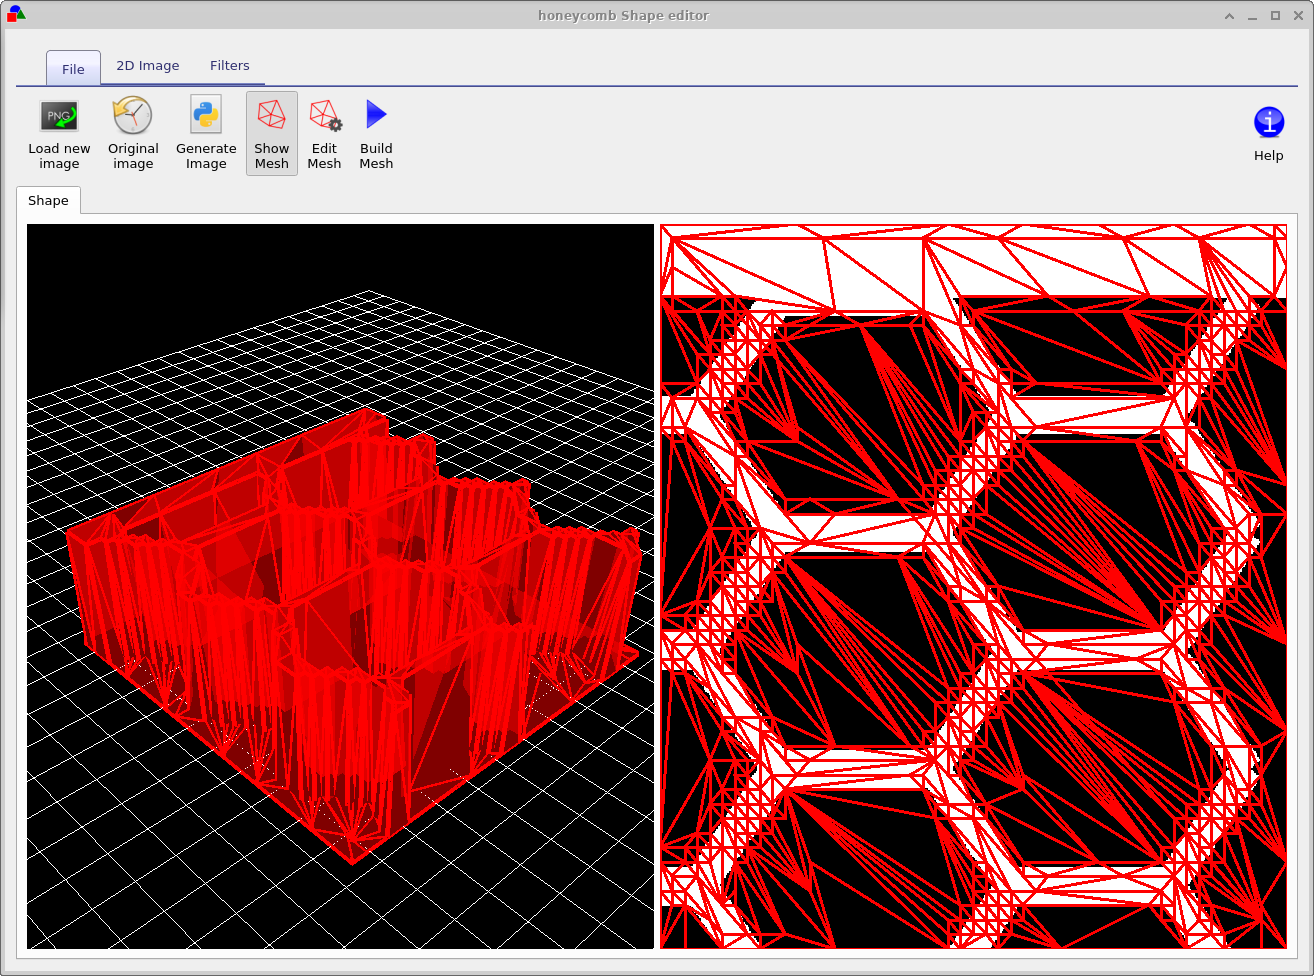
\includegraphics[width=\textwidth,height=0.7\textwidth]{./images/shape_db.png}
\caption{The shape database}
\label{fig:shapedb}
\end{figure}

\subsubsection{Filters database}
This contains optical filters.

